

To make our cycles represent flows of positive current,
coboundaries electrical potentials and resistance positive,
our sign conventions for arbitrarilly oriented labeled (multi)graphs
will be \emph{opposite that of} the homology of 1-dimensional chain complexes:
For $e : a \rightarrow b$, $\partial_1(e)=a-b$, $\partial^0(\hat{a})=\hat{e}+ \ldots\  $,
$\partial^0(\hat{b})=-\hat{e}+ \ldots\  $, where $e$ is edge with end vertices $a$ and $b$ oriented
as indicated\
\footnote{
On the other hand, for the sake of mathematical simplicity,
we will use this sign convention the port edges (in $P$) as well, unlike some electrical engineering
circuit theory writings in which the sign convention for ports only is reversed
so that quantities characterizing typical system behavior observable at the ports
are positive.}.
With $\partial^0(\phi(\hat{a}) \hat{a} + \phi(\hat{b}) \hat{b}) = (\phi(\hat{a})-\phi(\hat{b}))\hat{e} + \cdots$,
$\phi(\hat{a})-\phi(\hat{b})$ is the voltage drop going from $a$ to $b$.
Edge sets $E$ and $P$ will respectively represent resistors and ports.
When $e\in E$,
Ohm's law says the
$\phi(\hat{a})-\phi(\hat{b})$ times its resistance equals the current through $e$, flowing from $a$ to $b$.
For us, the currents through and voltage drops along
in all these edges are variables $i_t$ and $v_t$ for $t\in P\cup E$.  Ohm's law
is asserted in the homogeneous form:  For $e\in E$, the voltage-drop-to-current ratio
$v_e:i_e$ $=$ $r_e:g_e$, the ratio of the resistivity parameters.
Those parameters are not given for ports.
Kirchhoff's voltage law asserts that $\sum_tv_t\hat{t}$ is the 1-coboundry $\partial^0(\sum \phi(\hat{a})\hat{a})$
for some $\phi:V\rightarrow K$; physically, $\phi$ is the electrical potential function.
Kirchhoff's current law asserts that $\sum_ti_t t$ is a 1-cycle, i.e., in $\text{ker }\partial_1$. 
The problem of linear electrical network analysis is to characterize
the linear relationships among port current and voltage drop variables implied by
the network topology, Kirchhoffs' and Ohm's laws.  


Let $P=\{p_1, p_2\}$ and $E=\{e_1, e_2, e_3, e_4\}$ together be the edges in the (oriented) graph
below representing an electrical network, where $E$ represents the resistors.   $N_\alpha$ is
a full-row-rank, all-column submatrix of the matrix form for $\partial^1$.  It is the
usual ``signed'' vertex-edge incidence matrix which represents our graph's graphic matroid, with one
row deleted so $N_\alpha$ has full row rank.  The rows of $N_\alpha$ hold the coefficients in
Kirchhoff's current law, asserting that the edge currents constitute a 1-cycle, (i.e., a flow.)
$N_\beta^\perp$ is a totally unimodular matrix whose
rows are a basis for the 1-cycle space, conveniently
obtainable by coding the incidences of edges with the oriented fundamental
circuits each associated to an edge not in a fixed spanning tree.
Its rows hold the coefficients in
Kirchhoff's voltage law, asserting that the edge
voltages drops constitute a 1-coboundary, differences
of a potential along edges.
This well-known construction gives
two full row rank totally unimodular matrices whose row spaces are orthogonal complements,
representing our graph $G$'s
graphic (with bases $\mathcal{B}(G)$) and cographic matroids respectively.

\begin{figure}
  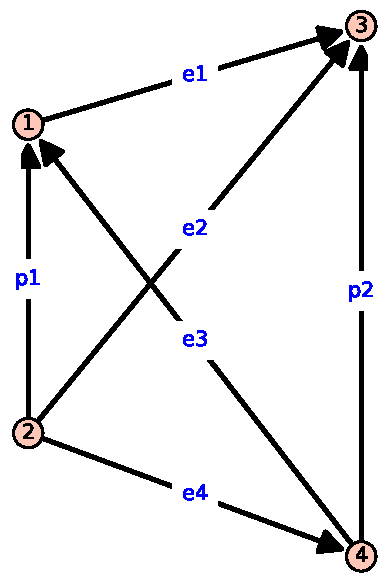
\includegraphics[scale=0.5]{K4.pdf}
\end{figure}


We form the following system of equations from (\ref{LmatrixDef}).
\[
N_\alpha=
\left(\begin{array}{cc|cccc}
1 & 0 & -1 & 0 & 1 & 0 \\
-1 & 0 & 0 & -1 & 0 & -1 \\
0 & 1 & 1 & 1 & 0 & 0
\end{array}\right)
%\]
\;\;\;\;
%\[
N_\beta^\perp =
\left(\begin{array}{cc|cccc}
1 & 0 & 0 & 0 & -1 & -1 \\
0 & 1 & 0 & -1 & 0 & 1 \\
0 & 0 & 1 & -1 & 1 & 1
\end{array}\right)
\]


%\[
%\left(\begin{array}{rrrrrr}
%1 & 0 & -g_{1} & 0 & g_{3} & 0 \\
%-1 & 0 & 0 & -g_{2} & 0 & -g_{4} \\
%0 & 1 & g_{1} & g_{2} & 0 & 0
%\end{array}\right)
%\]

%\[
%\left(\begin{array}{rrrrrr}
%1 & 0 & 0 & 0 & -r_{3} & -r_{4} \\
%0 & 1 & 0 & -r_{2} & 0 & r_{4} \\
%0 & 0 & r_{1} & -r_{2} & r_{3} & r_{4}
%\end{array}\right)
%\]

%\[
%\left(\begin{array}{cccccccc}
%  +1 & 0  & 0  & 0  & -g_{1} & 0     & +g_{3}  & 0 \\
%  -1 & 0  & 0  & 0  &  0    & -g_{2} & 0      & -g_{4} \\
%  0  & +1 & 0  & 0  & +g_{1} & +g_{2} & 0      & 0 \\
%  0  & 0  & +1 & 0  & 0     & 0      & -r_{3} & -r_{4} \\
%  0  & 0  & 0  & +1 & 0     & -r_{2}  & 0     & +r_{4} \\
%  0  & 0  & 0  & 0  & +r_{1} & -r_{2}  & +r_{3} & +r_{4}
%  \end{array}\right)
%\]
\begin{equation}\label{K4Equation}
\begin{split}
  0=L\left(\begin{array}{cc} {\Nal} \\ {\NbePe}  \end{array}\right)z
    =& \left[\begin{array}{c|c|c} \Nal(P)  &  0  &  \Nal(E)G \\  \hline
        0  & \NbePe(P)  &  \NbePe(E)R \end{array}\right]
    \left[ \begin{array}{c} i_{p_1} \\ i_{p_2} \\ v_{p_1} \\ v_{p_2} \\ x_{e_1} \\ x_{e_2} \\ x_{e_3} \\ x_{e_4}
      \end{array}
      \right]
    \\
    =&
\left(\begin{array}{cc|cc|cccc}
  1 & 0  & 0  & 0  & -g_{1} & 0     & g_{3}  & 0 \\
  -1 & 0  & 0  & 0  &  0    & -g_{2} & 0      & -g_{4} \\
  0  & 1 & 0  & 0  & g_{1} & g_{2} & 0      & 0 \\ \hline
  0  & 0  & 1 & 0  & 0     & 0      & -r_{3} & -r_{4} \\
  0  & 0  & 0  & 1 & 0     & -r_{2}  & 0     & r_{4} \\
  0  & 0  & 0  & 0  & r_{1} & -r_{2}  & r_{3} & r_{4}
  \end{array}\right)z
\end{split}
\end{equation}


The electrical network problem at hand is to determine linear constraints on the
port variables $i_p, v_p$, $p\in P = \{p_1, p_2\}$ imposed by the system.  In other words,
we want a linear map on the $U$-vector space with basis $P_\alpha, P_\beta$ whose kernel
is the projection of this system's solution space.

To compute $\ext{L}_E$, set 
$z=[\ext{p}_{\alpha 1},\ext{p}_{\alpha 2},\ext{p}_{\beta 1},\ext{p}_{\beta 2},
  \ext{e}_1,  \ext{e}_2,  \ext{e}_3,  \ext{e}_4]^t$
in the right hand side of (\ref{K4Equation}) 
and expand in terms of this basis
the exterior product (in order) of the resulting column's entries.
Finally, we select
the terms that can be expressed as $\ext{T}\ext{e}_1\ext{e}_2\ext{e}_3\ext{e}_4$.  The final
value is the sum of such $\ext{T}$.  Each $\ext{T}$ is a polynomial in the $g_e$, $r_e$
times the $\wedge$ of two distinct elements of
$\{\ext{p}_{\alpha 1}, \ext{p}_{\alpha 2}, \ext{p}_{\beta 1}, \ext{p}_{\beta 2}\}$.  Since each polynomial
term encodes a subset of $E=\{e_1, e_2, e_3, e_4\}$ (for example, $\{e_1, e_2\}$ is encoded
by $g_1g_2r_3r_4$) we take $r_e=1$, $e\in E$ to abbreviate the result. We call attention
to the fact that each polynomial enumerates
the common bases in a pair of our graph's matroid minors.


\begin{equation}\label{K4table}
\begin{array}{|c|c|c|} \hline
\text{basis element} & \text{coefficient} & \text{enumerates bases}\\
  \hline

\ext{p}_{\alpha 1}\ext{p}_{\alpha 2} &
g_1 + g_2 + g_3 + g_4 & \mathcal{B}(G/\{p_1, p_2\})

\\ \hline

\ext{p}_{\alpha 1}\ext{p}_{\beta 1} &
g_2g_3 - g_1g_4 &  \mathcal{B}(G/p_1\setminus p_2)\cap\mathcal{B}(G/p_2\setminus p_1)

\\ \hline

\ext{p}_{\alpha 1}\ext{p}_{\beta 2} &
(g_1 + g_2)(g_3 + g_4) & \mathcal{B}(G/p_1\setminus p_2)
\\ \hline 

\ext{p}_{\alpha 2}\ext{p}_{\beta 1} & -(g_1 + g_3)(g_2+g_4) & \mathcal{B}(G/p_2\setminus p_1)
\\ \hline
 
\ext{p}_{\alpha 2}\ext{p}_{\beta 2} &
-g_2g_3 + g_1g_4 & \mathcal{B}(G/p_1\setminus p_2)\cap\mathcal{B}(G/p_2\setminus p_1)
\\ \hline
 
\ext{p}_{\beta 1}\ext{p}_{\beta 2} &
g_1g_2g_3 + g_1g_2g_4 + g_1g_3g_4 + g_2g_3g_4 & \mathcal{B}(G\setminus \{p_1, p_2\})
\\ \hline

\end{array}
\end{equation}
